\section{Searching for Data Packages} \label{sec:searching}

Use Morpho searches to easily locate data packages (your packages and/or
packages shared by other scientists) based on a variety of specified
criteria. Packages can be searched by subject, taxonomic rank, and/or
spatial extent. Combine these major search criteria to further refine
result sets. 

Note: If you are not logged in to the KNB network but have network
access, the only network data packages that will appear in your search
results are those that have "public" access privileges. To view
additional data sets from the KNB network, log in to the KNB network
from the \hyperref[sec:main]{main Morpho screen}.

\subsection{Opening the Search Interface and Performing a Search}

To begin a search for data packages, do one of the following:
\begin{itemize}
  \setlength{\parskip}{1pt}
  \item click the search button
    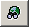
\includegraphics[scale=0.7]{images/button-search.png} found on the
    Toolbar on the \hyperref[sec:main]{main Morpho screen}.
  \item click ``Search for an existing data package'' on the
    \hyperref[sec:main]{main Morpho screen}.
  \item select ``Search'' from the \hyperref[sec:menu-search]{Search
    menu}.
\end{itemize}

The Morpho Search interface opens (\autoref{fig:search-main}), where you
can customize search criteria and specify the location of the files to
search.

\begin{figure}
  \centering
    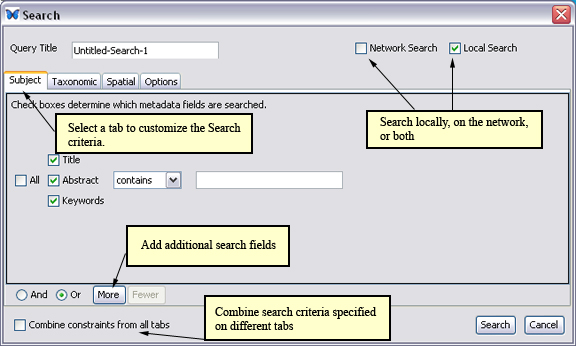
\includegraphics[width=0.7\textwidth]{images/search-main.jpg}
  \caption{The Morpho Search interface.}
  \label{fig:search-main}
\end{figure}

The four Search tabs (\nameref{sec:search-subject},
\nameref{sec:search-taxonomic}, \nameref{sec:search-spatial},
\nameref{sec:search-options}) allow users to search for specific text,
geographic extent, and taxonomic ranks and values. We'll talk about each
tab in more detail in the next few sections. Combine the criteria
specified on all four tabs to constrain your search so that it returns
only results that match all specified criteria. If the criteria are not
combined, the search will return data packages that match any specified
criteria. To combine criteria, check the "Combine constraints from all
tabs" box at the lower left of the Search interface. 

Check the appropriate boxes at the top right of the Search interface to
specify the search location: only locally (i.e., on your computer), in
the catalog (i.e., on the KNB network), or both.  Click "Search" to
perform the search at any time, or click "Cancel" to exit the Search
interface.

\subsubsection[Subject]{Subject search} \label{sec:search-subject}

Use the Subject tab (\autoref{fig:search-subject}) to search for
specific text in the data package documentation. To specify subject
criteria, type a search term in the space provided and select a metadata
field or fields to search (Title, Abstract, or Keywords). Choose whether
the field(s) contains, starts with, ends with, or equals the search
term. 

\begin{figure}
  \centering
    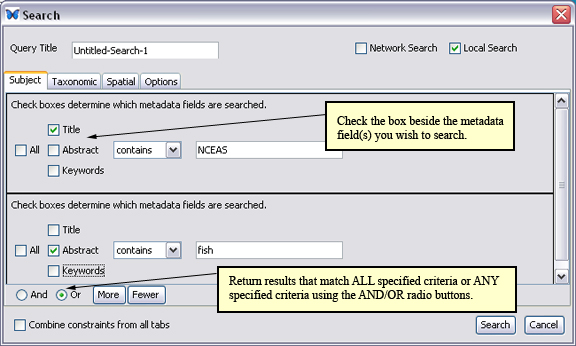
\includegraphics[width=0.7\textwidth]{images/search-subject.jpg}
  \caption{The Subject tab settings of the Search interface.}
  \label{fig:search-subject}
\end{figure}

To add fields for additional search terms, click the "More" button (the
"Fewer" button removes extra fields).  Use the And/Or radio buttons to
customize how results are returned. Choosing "And" returns only data
packages that match EVERY ONE of the specified search terms. Choosing
"Or" returns data packages that match ONE OR MORE of the specified
terms.

In \autoref{fig:search-subject}, the "More" button has been used to
create a second set of 'Subject' search criteria. The first set
instructs Morpho to look for items where the title starts with the
phrase "NCEAS". The second set indicates that the abstract should
contain the word "fish". These two search criteria are logically "OR"ed
with the radio button near the bottom of the screen.

\subsubsection[Taxonomic]{Taxonomic search} \label{sec:search-taxonomic}

Use the Taxonomic tab (\autoref{fig:search-taxonomic}) to search the
taxonomic metadata for data packages associated with a specified
taxonomic rank and value. Note that only taxonomic metadata fields are
searched; taxonomic information specified in other metadata fields
(e.g., keywords or title) is not considered by this search option. To
specify taxonomic criteria, type a taxon rank in the space provided and
select whether returned results contain, start with, end with, or equal
that value. For example, you can search for the taxon rank "Species",
and specify that the species name contains "Neotoma".

\begin{shaded}
  \textbf{NOTE} You can also include taxon synonyms from the Integrated
  Taxonomic Information System (ITIS) in the search using the setting
  under the \nameref{sec:search-options} tab.
\end{shaded}

\begin{figure}
  \centering
    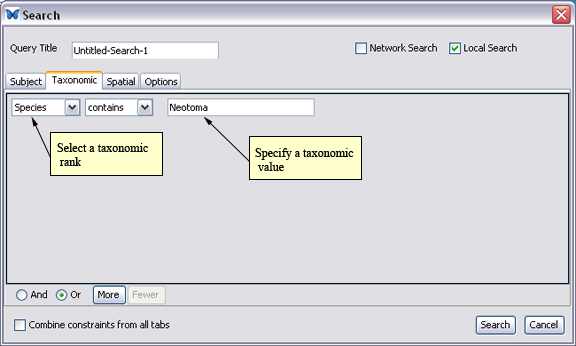
\includegraphics[width=0.7\textwidth]{images/search-taxonomic.jpg}
  \caption{The Taxonomic tab of the Search interface.}
  \label{fig:search-taxonomic}
\end{figure}

To add fields for additional taxon ranks, click the "More" button (the
"Fewer" button removes extra fields). Use the And/Or radio buttons to
customize how results are returned. Choosing "And" returns data packages
that match EVERY ONE of the specified search terms. Choosing "Or"
returns data packages that match ONE OR MORE of the specified terms.

\subsubsection[Spatial]{Spatial search} \label{sec:search-spatial}

The Spatial tab (\autoref{fig:search-spatial}) allows you to search for data packages
based on a specified geographic area. Morpho will return data packages
that contain geographic latitude/longitude coordinates inside (and
overlapping) the specified area.

\begin{figure}
  \centering
    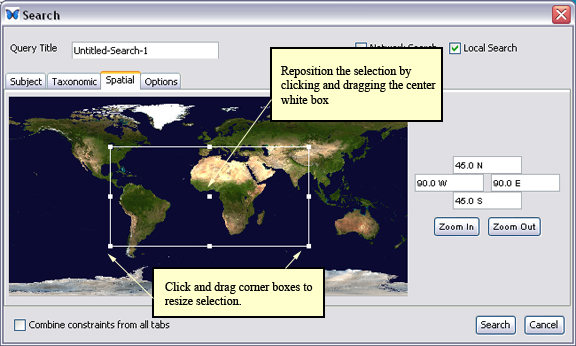
\includegraphics[width=0.7\textwidth]{images/search-spatial.jpg}
  \caption{The Spatial tab of the Search interface.}
  \label{fig:search-spatial}
\end{figure}

To manually draw a "bounding box" like the one displayed in
\autoref{fig:search-spatial}, click the map and then drag (with the
mouse still pressed). Release the mouse when the selection is complete.
Morpho will indicate the selection with a white rectangle and will note
the latitude and longitude values in the text boxes to the right of the
map. Use the white squares at the corners of the bounding box to resize
it. To reposition the selection, click and drag the white square in the
center.  To draw a more precise bounding box, zoom into an area of the
map using the "Zoom In" button. Return to the previous views using the
"Zoom Out" button. 

Coordinates of the bounding box can also be specified manually in the
text fields on the right side of the panel. Beginning with the top text
field and moving clockwise, these specify the north, east, south, and
west edges of the bounding box. Coordinates can be specified as the
number of degrees and the cardinal direction, as shown in
\autoref{fig:search-spatial}. If the number of degrees is entered
without a direction, positive numbers are treated as N or E, and
negative numbers as S or W. By default, values are specified in
fractional degrees. To enter degrees/minutes/seconds, type a space
between each value.

\subsubsection[Options]{Additional Options} \label{sec:search-options}

The Options tab (\autoref{fig:search-options}) allows you to specify whether the search should be
case-sensitive (i.e., only data packages matching the search term
exactly as it is specified will be returned). You can also choose to
include taxon synonyms from the Integrated Taxonomic Information System
(ITIS) in the search.  These two options can be saved as default
settings that will be applied to all future searches.

\begin{figure}
  \centering
    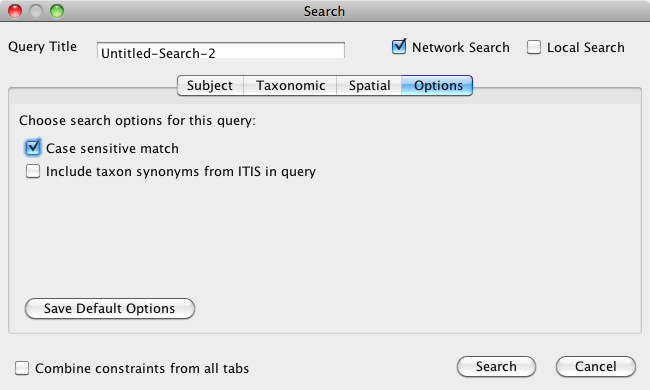
\includegraphics[width=0.7\textwidth]{images/search-options.png}
  \caption{The Options tab of the Search interface.}
  \label{fig:search-options}
\end{figure}

\subsection{Viewing Search Results}

Morpho displays the set of data packages that meets your search criteria
in the Search Results screen (\autoref{fig:search-results}). The
interface indicates whether the packages consist of only metadata or
metadata and data, as well as whether the packages are located on the
local machine, the network, or both.

To open a data package and view it, do one of the following:
\begin{itemize}
  \setlength{\parskip}{1pt}
    \item double-click the package,
    \item right-click the package and select "Open" from the menu,
    \item select the desired data package, and then click the "Open"
      button in the Toolbar at the top of the window.
\end{itemize}

You can also open an earlier version of the data package (if any exist)
by right-clicking and selecting "Open Previous Version." Note that one
or more previous versions of the data package may be unavailable, for
example, a version saved only locally on a different computer.

\begin{figure}
  \centering
    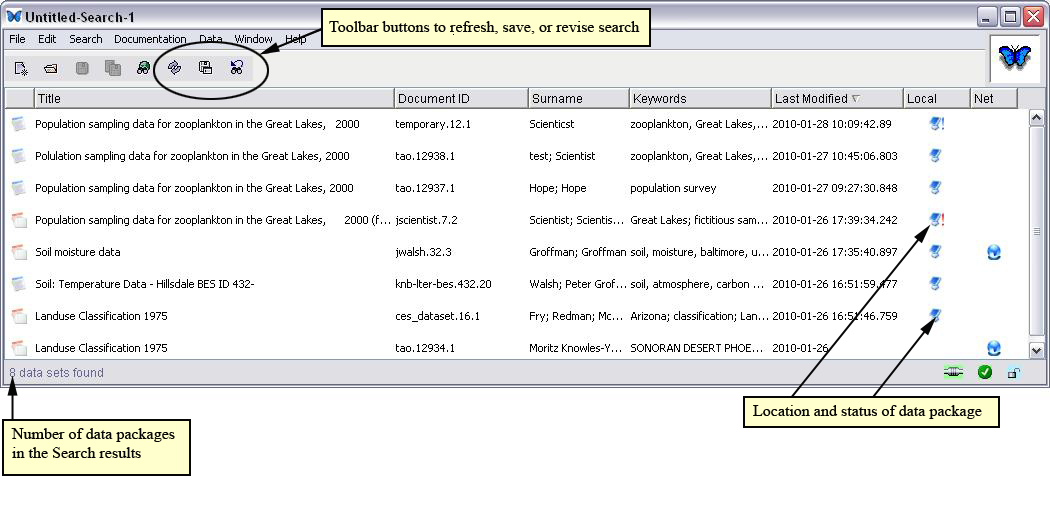
\includegraphics[width=0.7\textwidth]{images/search-results.jpg}
  \caption{Search results displayed in the Morpho interface.}
  \label{fig:search-results}
\end{figure}

The icons in the first column of the Open Data Package screen tell you
if the package contains:
\begin{itemize}
  \parskip 3pt
  \itemsep 0pt
  \item[] 
\includegraphics[scale=0.7]{images/indicator-hasdata.png}
    Data and documentation
  \item[] 
\includegraphics[scale=0.7]{images/indicator-hasnodata.png}
	Documentation only 
\end{itemize}

Icons in the last two columns indicate the location and status of the
package:
\begin{itemize}
  \parskip 3pt
  \itemsep 0pt
  \item[] 
\includegraphics[scale=0.7]{images/indicator-dp-local.png}
  Local data package
  \item[] 
\includegraphics[scale=0.7]{images/indicator-dp-incomplete.png}
  Saved incomplete data package
  \item[] 
\includegraphics[scale=0.7]{images/indicator-dp-network.png}
  Network data package
  \item[] 
\includegraphics[scale=0.7]{images/indicator-dp-recovered.png}
  Recovered incomplete data package
\end{itemize}

For more information about saved and recovered incomplete data package,
please see \autoref{sec:dp-saveforlater} and
\autoref{sec:dp-recover}.

Use the Morpho Toolbar buttons to refresh the search, save the search
for future use, or revise the search by changing the search parameters
(\autoref{fig:buttons-post-search}). These options are also available
from the main Search menu located at the top of each screen.

\begin{figure}
  \centering
    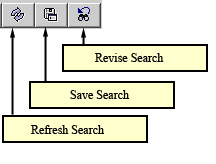
\includegraphics[width=0.4\textwidth]{images/buttons-post-search.jpg}
  \caption{Toolbar buttons for search results.}
  \label{fig:buttons-post-search}
\end{figure}

\subsection{Saving a Search}

To save a search and its parameters for later use, specify a name for
the search in the "Query Title" field, and then save the search by
clicking the "Save search" button in the Toolbar, or by selecting "Save
Search" from the Search menu. Saved searches are accessed directly from
the Search menu (\autoref{fig:search-saved}).

\begin{figure}
  \centering
    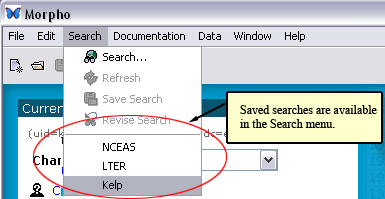
\includegraphics[width=0.7\textwidth]{images/search-saved.jpg}
  \caption{Access saved searches from the Search menu.}
  \label{fig:search-saved}
\end{figure}

\begin{shaded}
  \textbf{NOTE} You cannot delete a saved search via the Morpho
  interface. To remove a saved search, look in the
  \texttt{.morpho/profiles/<profilename>} directory and delete the
  "queries" subdirectory to remove all queries, or one of the files in
  the queries subdirectory to remove that search.
\end{shaded}

